\documentclass[
    a5paper,
    pagesize,
    11pt,
    bibtotoc,
    normalheadings,
    twoside,
    openany,
    chapterprefix,
    DIV=9
]{scrbook}

\usepackage[utf8]{inputenc}
\usepackage{tocloft}
\usepackage{mathtools}
\usepackage{amsfonts}
\usepackage{enumitem}
\usepackage{amsmath}
\usepackage{amsthm}
\usepackage{amssymb}
\usepackage[hmargin=2cm, vmargin=2.5cm]{geometry}
\usepackage{graphicx}
\usepackage{wrapfig}
\usepackage{parskip}
\usepackage{framed}
\usepackage{fancyhdr}
\usepackage{emptypage}
\usepackage{multicol}
\usepackage{imakeidx}
\usepackage[breaklinks]{hyperref}
\usepackage[capitalise, nameinlink]{cleveref}
\usepackage[x11names]{xcolor}
\usepackage{crossreftools}

\usepackage[
    backend=bibtex,
    style=alphabetic,
    sorting=ynt
]{biblatex}

%=========== Path to images ==============
\graphicspath{{./images/}}

%============== Resources ================
\addbibresource{../abstract-algebra.bib}

%============ Redefinitions ==============
\let\oldemptyset\emptyset
\let\emptyset\varnothing

\let\totient\varphi

\renewcommand{\vert}{ \ \vline \ }
\newcommand{\vertalt}{ \ | \ }

\newcommand{\myref}[1]{\textbf{\crthypercref{#1}}}
\newcommand{\myreffigures}[1]{\textbf{\cref{#1}}}

\renewcommand{\qedsymbol}{\ensuremath{\blacksquare}}

%=========== Theorem Styles ==============
\newtheoremstyle{theorem-style}
    {-12pt}      % Space above
    {-5pt}       % Space below
    {}           % Font to use in the theorem
    {0pt}        % Measure of space to indent
    {\bfseries}  % Name of the head font
    {.}          % Punctuation between head and body
    { }          % Space after theorem head; " " = normal inter-word space
    {\thmname{#1}\thmnumber{ #2}\textit{\thmnote{ (#3)}}}

\newtheoremstyle{definition-style}
    {-12pt}      % Space above
    {-5pt}       % Space below
    {}           % Font to use in the definition
    {0pt}        % Measure of space to indent
    {\bfseries}  % Name of the head font
    {.}          % Punctuation between head and body
    { }          % Space after theorem head; " " = normal inter-word space
    {\thmname{#1}\thmnumber{ #2}\textnormal{\thmnote{ (#3)}}}

\newtheoremstyle{exercise-style}
    {-5pt}       % Space above
    {\topsep}    % Space below
    {}           % Font to use in the exercise
    {0pt}        % Measure of space to indent
    {\bfseries}  % Name of the head font
    {.}          % Punctuation between head and body
    { }          % Space after theorem head; " " = normal inter-word space
    {\thmname{#1}\thmnumber{ #2}\textnormal{\thmnote{ (#3)}}}

%======== Theorem-Like Things ============
\theoremstyle{theorem-style}\newtheorem{theoremhidden}{Theorem}[section]
\renewcommand{\thetheoremhidden}{\Roman{part}.\arabic{chapter}.\arabic{section}.\arabic{theoremhidden}}

\theoremstyle{theorem-style}\newtheorem{lemmahidden}[theoremhidden]{Lemma}

\theoremstyle{theorem-style}\newtheorem{propositionhidden}[theoremhidden]{Proposition}

\theoremstyle{theorem-style}\newtheorem{corollaryhidden}[theoremhidden]{Corollary}

\theoremstyle{definition-style}\newtheorem{definitionhidden}[theoremhidden]{Definition}

\theoremstyle{exercise-style}\newtheorem{exercisehidden}{Exercise}[chapter]
\renewcommand{\theexercisehidden}{\Roman{part}.\arabic{chapter}.\arabic{exercisehidden}}

\theoremstyle{definition}\newtheorem{problem}{Problem}[chapter]
\renewcommand{\theproblem}{\Roman{part}.\arabic{chapter}.\arabic{problem}}

\theoremstyle{definition}\newtheorem*{remark}{Remark}
\theoremstyle{definition}\newtheorem{example}[theoremhidden]{Example}

%============ Environments ===============
% 'Results' environments
\newenvironment{theorem}
{\definecolor{shadecolor}{named}{DarkSeaGreen2}\begin{shaded}\noindent\begin{theoremhidden}}
{\end{theoremhidden}\end{shaded}}

\newenvironment{lemma}
{\definecolor{shadecolor}{named}{Honeydew2}\begin{shaded}\noindent\begin{lemmahidden}}
{\end{lemmahidden}\end{shaded}}

\newenvironment{proposition}
{\definecolor{shadecolor}{named}{Honeydew1}\begin{shaded}\noindent\begin{propositionhidden}}
{\end{propositionhidden}\end{shaded}}

\newenvironment{corollary}
{\definecolor{shadecolor}{named}{DarkSeaGreen1}\begin{shaded}\noindent\begin{corollaryhidden}}
{\end{corollaryhidden}\end{shaded}}

\newenvironment{definition}
{\definecolor{shadecolor}{named}{LightCyan1}\begin{shaded}\noindent\begin{definitionhidden}}
{\end{definitionhidden}\end{shaded}}

\newenvironment{exercise}
{\begin{framed}\noindent\begin{exercisehidden}}
{\end{exercisehidden}\end{framed}}

% 'Questions' environments
\newenvironment{questions}
{\begin{enumerate}[label=\textbf{\arabic*.}]}
{\end{enumerate}}

\newenvironment{partquestions}[1]
{\begin{enumerate}[label=\textbf{(#1)}]}
{\end{enumerate}}

%=========== Custom Commands =============
\newcommand{\code}[1]{\texttt{#1}}  % Code block
\makeatletter\newcommand*{\rom}[1]{\Ifstr{#1}{0}{0}{\expandafter\@slowromancap\romannumeral #1@}}\makeatother  % Roman numeral

\newcommand{\lcm}{\mathrm{lcm}}  % Lowest common multiple function
\newcommand{\sgn}{\mathrm{sgn}}  % Signum function

\newcommand{\im}{\mathrm{im}\;}  % Image of a function
\newcommand{\id}{\mathrm{id}}    % Identity function

%======== Custom Chapter Styling =========
\makeatletter
\renewcommand{\chaptermark}[1]{
    \markboth{\if@mainmatter\chapapp~\thechapter.\ \fi#1}{}
}

\renewcommand*{\chapterformat}{
  \MakeUppercase{\chapapp\nobreakspace\thechapter}
}

\renewcommand*{\chapterlineswithprefixformat}[3]{
    \Ifstr{#1}{chapter}{
        \vspace{-60px}
        \Ifstr{#2}{\empty}{\vspace{40px}}{\raggedleft#2}
        \vspace{-15px}
        \rule{\linewidth}{1pt}\par\nobreak
        \centering{#3}
        \vspace{-10px}
        \rule{\linewidth}{1pt}\par\nobreak
        \vspace{-10px}
    }{#2#3}
}
\makeatother

%======== Figure Caption Format ==========
\usepackage[labelfont=bf]{caption}
\DeclareCaptionLabelFormat{custom}{#1 \Roman{part}.#2.}
\captionsetup{labelformat=custom,labelsep=space}

%============ Custom Header ==============
\fancypagestyle{plain}{\fancyhf{}\renewcommand{\headrulewidth}{0pt}}  % To clear page numbers from footer, and header line at the start of every chapter

\pagestyle{fancy}
\fancyhf{}  % Clear header/footer

\fancyhead[LE,RO]{\thepage}
\fancyhead[LO,RE]{\textit{\nouppercase\leftmark}}

%========= Customise TOC Heading =========
\makeatletter
\def\createtoc{
    \renewcommand\tableofcontents{
        \chapter*{\contentsname}
        \@starttoc{toc}
    }
    \tableofcontents
}
\makeatother

%======= Customise Draft Watermark =======
\newcommand{\setasdraft}{
    \usepackage{draftwatermark}
    \SetWatermarkLightness{0.95}
    \SetWatermarkScale{5}
}

%========= Front Matter Pages ============
\def\volumetitle{Volume \rom{\volumenumber}: \volumename}

\def\frontmatterpages{
    \frontmatter  % Use lowercase roman numerals for page numbers

    % Title page
    \begin{titlepage}
        \centering{
            \selectfont
            \Huge
            \textbf{Abstract Algebra}\\
            \vspace{-0.2cm}
            
            \Large
            \textbf{A Simple Introduction}\\
            \vspace{0.5cm}
            
            \LARGE
            \volumetitle
            \vspace{2cm}
        }\\
        \centering{\Large{Overwrite}}
        \vspace{\fill}

        \includegraphics[width=5cm]{\volumeimage}
        \vspace{\fill}

        \centering \small{\textit{Version \version}}
    \end{titlepage}

    \newpage{}

    % Edition notice
    \clearpage\null\vfill
    \thispagestyle{empty}
    \begin{minipage}[b]{0.9\textwidth}
        \footnotesize\raggedright
        \setlength{\parskip}{0.5\baselineskip}

        Published by Kan Onn Kit\\
        Singapore
        \vspace{5cm}

        \textbf{Abstract Algebra: A Simple Introduction -- \volumetitle}\par
        Version \version
        \vspace{0.3cm}

        Copyright \copyright \ 2022 -- \the\year\ by Kan Onn Kit\par
        This work is licensed under a
        Creative Commons Attribution-NonCommercial-ShareAlike 4.0 International Licence.\par
        
\includegraphics[width=2.5cm]{../images/CC_BY-NC-SA_4.0.png}\\  % With reference to the volumes' folders
        The full licence text is available at \url{http://creativecommons.org/licenses/by-nc-sa/4.0/}.\par    
        The source files for the project are available \href{https://github.com/PhotonicGluon/Abstract-Algebra-Book}{here}.
        \vspace{0.3cm}

        Typeset in 11pt Computer Modern Roman using PDF\LaTeX.
    \end{minipage}

    \vspace*{2\baselineskip}
    \cleardoublepage

    % "Quote" page
    \thispagestyle{empty}
    \vspace*{2cm}

    \begin{center}
        \Large{\parbox{10cm}{
            \begin{raggedright}
                \Large
                \quotepagetext
                \vspace{0.3cm}
                
                \hfill
                --- \quotepageattribution\\
                \vspace{-0.25cm}
                
                \hfill
                \normalsize
                (\quotepagecitation)
            \end{raggedright}
        }
    }
    \end{center}

    \newpage

    % Table of contents
    \createtoc
    \setcounter{part}{\volumenumber}

    % Acknowledgements
    \chapter{Acknowledgements}
    Undertaking such a monumental project is new to me, and I am indebted to the people who accompanied me on this journey.

    I am eternally grateful to my parents, who have spent countless hours and an ungodly amount of effort to raise me into who I am today. Their omnipresent kindness, patience, and love for me are something I certainly do not deserve, and I thank them for taking care of me.
    
    I would like to thank my tutor Leong Chong Ming, who got me interested in abstract algebra in the first place. His enthusiasm and eagerness in sharing his knowledge on the subject is the driving force behind my decision to write these books.

    I am grateful for the help of my friend Low Ji Yuan, who has assisted me with countless revisions of the content in these books and given me another pair of eyes in the vetting of content.

    I also sincerely appreciate the support from my mathematics tutors, Loke Weng Heng, Siow Yun Jie, and Teng Yen Ping, who has been there through my junior college years inspiring me with the wonders of mathematics. I am indebted to them for allowing me to excel in my final examinations.

    My close friends, Aidan Tay, Gabriel Fong, and Low Ji Yuan, accompanied me through two years of schooling (and math jokes). I offer infinite thanks to them for sticking with me and for encouraging this math nerd to pursue his wacky projects.

    A thousand thanks go out to my teachers at the School of Science and Technology, Singapore, and specifically my form teacher Lee Tsi Yew Samuel, who instilled important character values into me so I can excel in my future endeavours.

    % Preface
    \chapter{Preface}
    Although algebra has a long history, it has undergone quite striking changes in the past few decades. Abstract (or modern) algebra is widely recognised as an essential element of higher mathematical education. The results that it showcases, however, are often hard to grasp and understand without prerequisite knowledge or with a heavy background in mathematics. Most books on this subject are crafted for undergraduates at universities. They are not for a general mathematics enthusiast or one who seeks to understand more about the inner structure of algebra that mathematicians encounter frequently.

    The exploration of such structures is fundamental to the current underpinning of scientific inquiries. For example, groups are important as they describe the symmetries which the laws of physics seem to obey. Finite fields are also used in coding theory and combinatorics. I hope this series of books will inspire more people to learn more about abstract algebra, beyond the simple introduction presented here.

    This series of books serves to achieve several goals.
    \begin{itemize}
        \item Provide a step-by-step explanation of core results from abstract algebra, without ambiguity of the results discussed.
        \item Demystify the core steps that many textbooks skip over when writing proofs.
        \item Ensure that results from abstract algebra are as accessible, as approachable, and as understandable for as many people as possible.
    \end{itemize}
    I hope that these books can accomplish these goals and let readers enjoy the wonders of abstract algebra.

    \hfill{\textit{22 March, 2023}}

    \section*{Preface for Volume \rom{\volumenumber}}
    \prefacevolumetext
    
    \hfill{\textit{\prefacevolumedate}}

    % Suggestions on the use of this book
    \chapter{Suggestions on the Use of This Book}
    \section*{General Information}
    \begin{itemize}
        \item For most volumes, we include both exercises and problems.
        \begin{itemize}
            \item An exercise can be thought of as a simple ``self-review'' question. Exercises ensure that the content of a particular section is understood and should not be too hard to answer.
            \item A problem is a more holistic version of an exercise. Generally, solutions to problems require a thorough understanding of the current chapter and may require results from other chapters.
        \end{itemize}
        \item A consistent labelling system for all the results within and between volumes is necessary for a project as long as this one.
        \begin{itemize}
            \item All definitions, examples, lemmas, theorems, propositions, and corollaries are consecutively numbered, using the format
            \begin{quote}
                \code{[VOLUME].[CHAPTER].[SECTION].[NUMBER]}
            \end{quote}
            For example, the fourth statement in Volume I, chapter 2, section 3 is labelled \textbf{I.2.3.4}.
            \item Exercises and problems are also numbered consecutively, using the format
            \begin{quote}
                \code{[VOLUME].[CHAPTER].[NUMBER]}
            \end{quote}
            For example, the third exercise in Volume I, chapter 2 is labelled \textbf{I.2.3}. Likewise, the fourth exercise in Volume II, chapter 3 is labelled \textbf{II.3.4}.
        \end{itemize}
        \item Volume numbers are always written in Roman numerals, except for Volume 0 which will be written as a zero.
        \item The symbol ``$\qedsymbol$'' marks the end of a proof.
    \end{itemize}

    \section*{Chapter Interdependence}
    The diagram on the next page shows chapter interdependence. It should be used in conjunction with the table of contents and notes listed.

    \newpage
    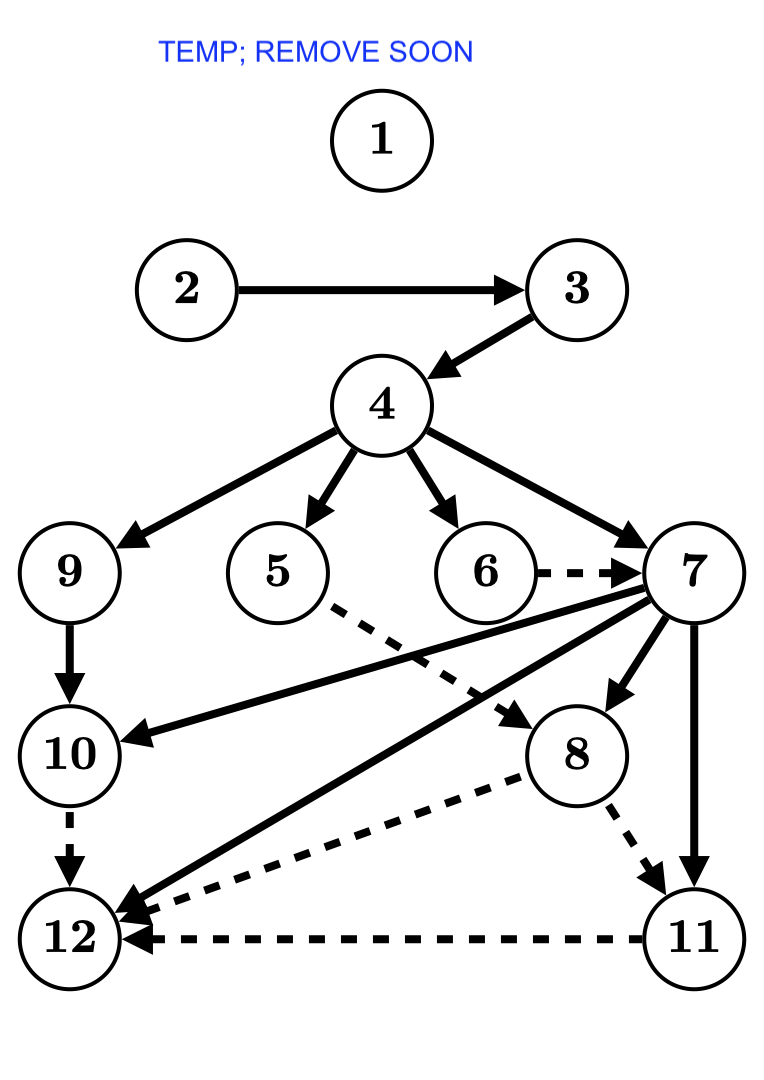
\includegraphics[width=\linewidth]{interdependence.png}
    
    \newpage

    \textbf{Notes}:
    \interdependencenotes

    \mainmatter  % Now use arabic numerals for page numbers
}

%============= Index Pages ===============
\usepackage[
    totoc,
    columnsep=20pt,
    hangindent=8pt,
    subindent=20pt,
    subsubindent=30pt
]{idxlayout}

\makeindex[options= -s ../index-style.ist]

%======= Bibliography Formatting =========
% These two lines are here to ensure that URLs do not exceed the page by too much
\setcounter{biburllcpenalty}{7000}
\setcounter{biburlucpenalty}{8000}
